%!TEX root = Slic3r-Manual.tex

\section{Hauteur de couche variable} % (fold)
\label{sec:variable_layer_height}
\index{layer height}
\index{hauteur de couche}

Slic3r donne la possibilité de régler la hauteur de couche entre des positions arbitraires le long de l'axe Z. Voilà, des parties du modèle peuvent être imprimés avec une hauteur de couche grossière, par exemple des sections verticales, et d'autres parties pourraient être imprimés avec une hauteur de couche plus fine, par exemple les dégradés inclinés où les couches apparaissent plus marquées.

Le modèle de la fig. \ref{fig:example_model} donne un exemple rudimentaire où des hauteurs de couche variables pourraient être utilisées pour améliorer la qualité d'impression.  Les murs de la structure n'ont pas à être imprimés en haute définition pour une qualité acceptable, mais la pente du toit apparait en escalier, une hauteur de couche de 0,4 mm est trop grossière, en particulier pour la couche supérieure, qui est aplatie.  Ceci est illustré dans le G-Code représenté à la fig \ref{fig:example_gcode_normal_layer_heights}.


\begin{figure}[H]
\centering
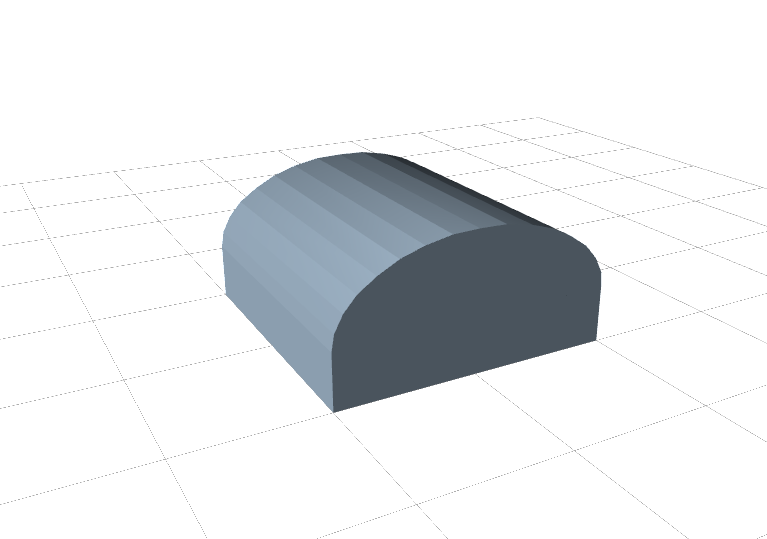
\includegraphics[keepaspectratio=true,width=0.75\textwidth]{expertmode/variable_layer_height/example_model.png}
\caption{Exemple de modèle mettant en evidence un cas d'utilisation des couches variables.}
\label{fig:example_model}
\end{figure}

\begin{figure}[H]
\centering
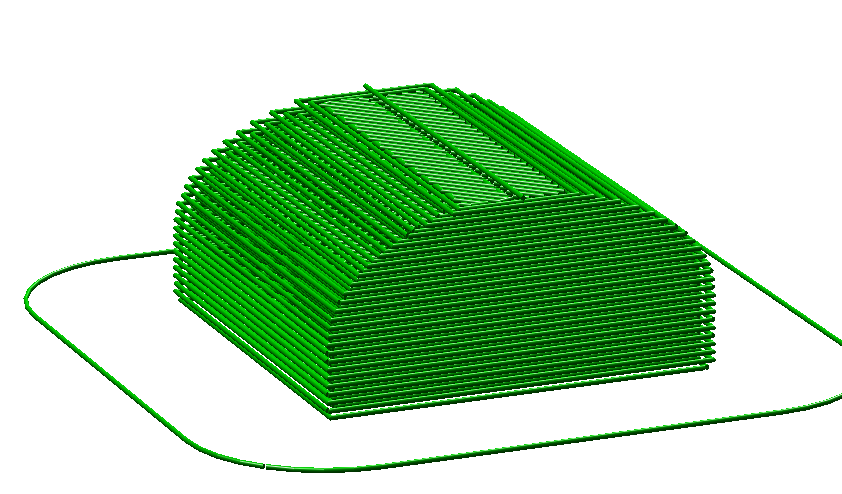
\includegraphics[keepaspectratio=true,width=0.75\textwidth]{expertmode/variable_layer_height/example_gcode_normal_layer_heights.png}
\caption{Exemple avec des couches normales.}
\label{fig:example_gcode_normal_layer_heights}
\end{figure}

Les paramètres de hauteur de couche variables sont disponibles en double-cliquant sur ​​le nom de la pièce dans la fenêtre Plater (surface de travail).  Cela ouvrira une fenêtre qui contient deux onglets. Le premier donne des informations sur le modèle, comme indiqué dans la fig. \ref{fig:variable_layer_height_options_tab_1}.

\begin{figure}[H]
\centering
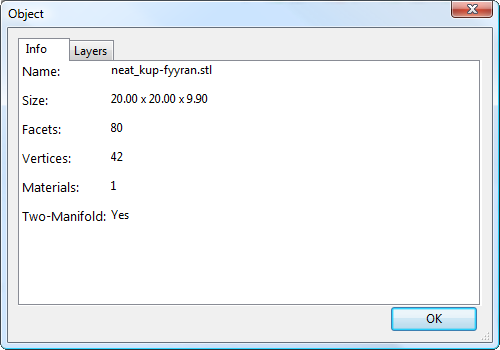
\includegraphics[keepaspectratio=true,width=0.75\textwidth]{expertmode/variable_layer_height/variable_layer_height_options_tab_1.png}
\caption{Paramètres de Couche variable - Info.}
\label{fig:variable_layer_height_options_tab_1}
\end{figure}

Il convient de noter la hauteur du modèle, puisque cela sera utile pour le calcul de la hauteur maximale de Z.

Le deuxième onglet (fig. \ref{fig:variable_layer_height_options_tab_2}) présente un tableau dans lequel chaque rangée définit une hauteur de couche pour une plage particulière le long de l'axe Z, exprimée en millimètres. Dans cet exemple, les parois du modèle sont imprimés à 0,4 mm, les parties raides du toit sont imprimées à 0,2 mm, et la moins raide à 0,15 mm. Notez que chaque plage se divise exactement par la hauteur de la couche donnée de sorte qu'il n'y a pas de «trous» entre les sections.

\begin{figure}[H]
\centering
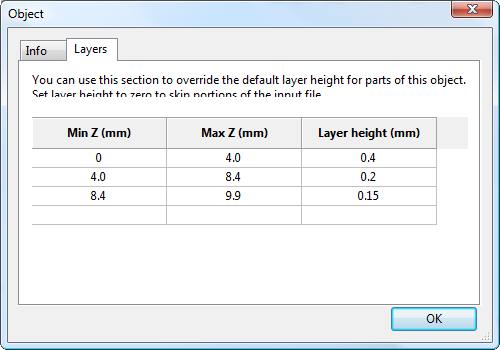
\includegraphics[keepaspectratio=true,width=0.75\textwidth]{expertmode/variable_layer_height/variable_layer_height_options_tab_2.png}
\caption{Paramètres de Couche variable - Layers (Couches).}
\label{fig:variable_layer_height_options_tab_2}
\end{figure}

Le G-Code résultant (fig. \ref{fig:example_gcode_variable_layer_heights}) montre une plus haute définition qui devrait aboutir à une impression de qualité supérieure.

\begin{figure}[H]
\centering
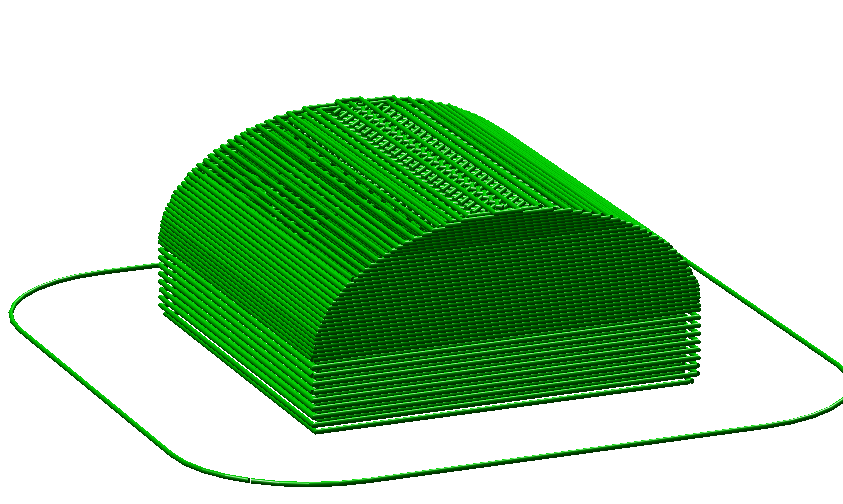
\includegraphics[keepaspectratio=true,width=0.75\textwidth]{expertmode/variable_layer_height/example_gcode_variable_layer_heights.png}
\caption{Example avec une hauteur de couche variable.}
\label{fig:example_gcode_variable_layer_heights}
\end{figure}

La Fig. \ref{fig:example_print} montre le modèle d'exemple imprimé.  L'impression de la gauche a 0,4 mm hauteur de la couche partout, alors que l'impression sur la droite a la hauteur de la couche variable.

\begin{figure}[H]
\centering
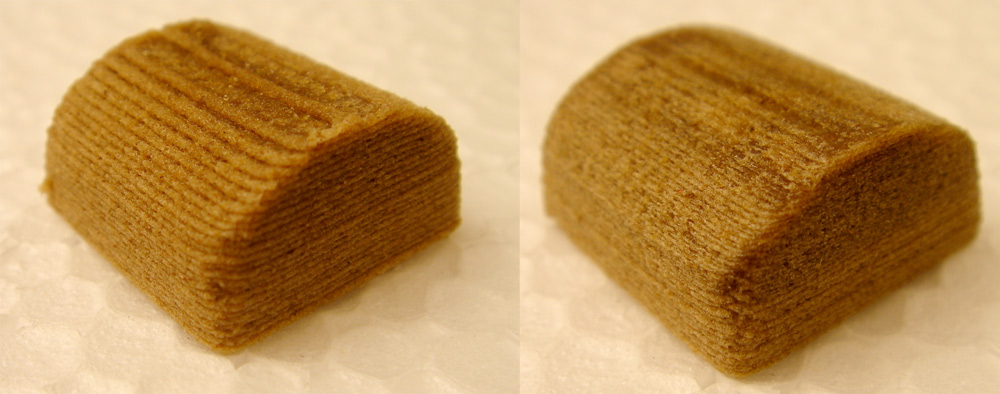
\includegraphics[keepaspectratio=true,width=1\textwidth]{expertmode/variable_layer_height/example_print.jpg}
\caption{Exemple d'impression avec une hauteur de couches variable.}
\label{fig:example_print}
\end{figure}

Une caractéristique supplémentaire de l'option de hauteur de couches variable est que par la saisie d'un zéro pour une plage de la partie du modèle ne sera pas imprimé.  Fig. \ref{fig:example_gcode_skipped_layers} shows the G-Code where layers between 0 and 4mm are skipped.  This is a useful way of dividing a tall model into multiple, shorter sections which can be printed individually and assembled afterwards.
\begin{figure}[H]
\centering
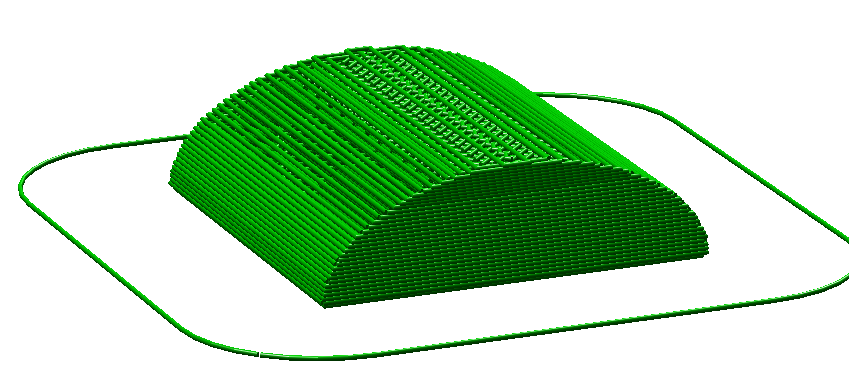
\includegraphics[keepaspectratio=true,width=0.75\textwidth]{expertmode/variable_layer_height/example_gcode_skipped_layers.png}
\caption{Exemple avec des couches ignorés.}
\label{fig:example_gcode_skipped_layers}
\end{figure}

% section variable_layer_height (end)